\setchapterpreamble[u]{\margintoc}
\chapter{Answers}
\labch{ch-answers}


Tasks and questions are scattered throughout the book, 
and the answers are collected in this chapter.


\section{Introduction}
\labsec{answer-intro}


\begin{exercise}%
    \label{answer:short-link-to-SPARQL}
How to create a short link to a SPARQL script?
\end{exercise}

\begin{marginfigure}[0cm]
    {%
        \setlength{\fboxsep}{0pt}
        \setlength{\fboxrule}{1pt}
        \fcolorbox{gray}{gray}{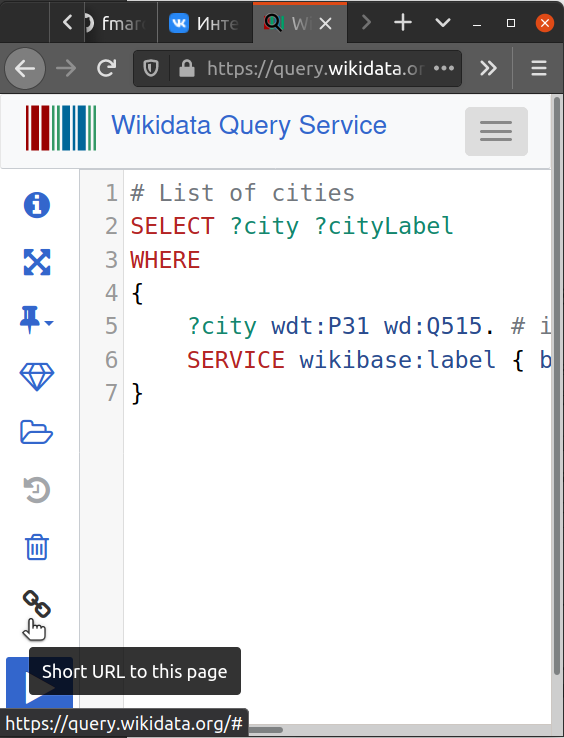
\includegraphics[width=\linewidth]{chapter/intro/WD_Query_Service_Short_URL_2020.png}}
    }
	\caption{The chain symbol button creates a short link to the SPARQL script, Wikidata Query Service, 2020.}
	\labfig{fig:WDQS-Short-URL-creation}
\end{marginfigure}

The Wikidata Query Service is shown in~\reffig{fig:WDQS-Short-URL-creation}. 
The bottom button with a chain symbol allows you to create a short link to the SPARQL script. 

See question on page~\pageref{question:short-link-to-SPARQL}.



\section{Aircraft from small to large}
\labsec{answer-aircraft}

%%%%%%%%%%%%%%%%%%%%%%%%%%%%answer_1%%%%%%%%%%%%%%%%%%%%%%

\begin{exercise}%
    \label{answer:aircraft_manufacturers_en}
Which Russian aircraft manufacturers have websites?
\begin{itemize}
\item MiG
\item Saratov Aviation Plant
\item Tupolev
\item Sukhoi
\end{itemize}
\end{exercise}

The following Russian manufacturers have websites: Mig, Tupolev and Sukhoi. The answer to the question can also be obtained by running the following SPARQL query (listing~\ref{lst:aircraft_listing_Manufacturers_websites}). 
    
\begin{lstlisting}[ language=SPARQL, breaklines=true, 
                    caption={Manufacturers websites\\\hspace{\textwidth}
                        SPARQL query: \href{https://w.wiki/rg8}{w.wiki/rg8}
                        },
                    label=lst:aircraft_listing_Manufacturers_websites,
                    texcl 
                    ]
SELECT ?manufacturer ?manufacturerLabel ?site
WHERE
{
    ?manufacturer wdt:P31 wd:Q936518. # instance of aerospace manufacturer
  	?manufacturer wdt:P17 wd:Q159. # country Russia
  	?manufacturer wdt:P856 ?site # official website
    SERVICE wikibase:label { bd:serviceParam wikibase:language "en" }
}
\end{lstlisting}

Question from page~\pageref{question:aircraft_manufacturers_en}.

%%%%%%%%%%%%%%%%%%%%%%%%%%%%answer_2%%%%%%%%%%%%%%%%%%%%%%

\begin{exercise}%
    \label{answer:aircraft_answer_2}
Find the correspondence between the date of foundation and the company.
\\
\begin{tabular}{ l | l }
Company & Foundation date \\ \hline
MiG & 01.01.1939 \\
Vympel & 18.11.1949 \\
Tupolev & 18.12.1939 \\
Sukhoi & 01.01.1922 \\
\end{tabular}
\end{exercise}

The company ``Mig" was founded on December 18.1939, ``Pennant" - November 18.1949, ``Tupolev" - January 01.1922, ``Sukhoi" - January 01.1939 Reply the question can also be obtained by running the following SPARQL-request (listing \ref{lst:aircraft_company_foundation_date_lst_en}). 
       
\begin{lstlisting}[ language=SPARQL, breaklines=true, 
                    caption={Company foundation dates\\\hspace{\textwidth}
                        SPARQL query: \href{https://w.wiki/rg7}{w.wiki/rg7}
                        },
                    label=lst:aircraft_company_foundation_date_lst_en,
                    texcl 
                    ]
SELECT ?manufacturer ?manufacturerLabel ?inception
WHERE
{
    ?manufacturer wdt:P31 wd:Q936518. # instance of aerospace manufacturer
  	?manufacturer wdt:P17 wd:Q159. # country Russia
  	?manufacturer wdt:P571 ?inception # foundation date
    SERVICE wikibase:label { bd:serviceParam wikibase:language "en" }
}
\end{lstlisting}

Question from page~\pageref{question:aircraft_question_2}.

%%%%%%%%%%%%%%%%%%%%%%%%%%%%answer_3%%%%%%%%%%%%%%%%%%%%%%

\begin{exercise}%
    \label{answer:aircraft_company_headquarters_en}
Find the correspondence between the location of the company's headquarters and the company.
\\
\begin{tabular}{ l | l }
Company & Headquarters \\ \hline
Kazan Helicopters Plant & Kazan \\
Saratov Aviation Plant & Saratov \\
Ulan-Ude Aviation Plant & Ulan-Ude \\
Sukhoi & Moscow \\
\end{tabular}
\end{exercise}

The headquarters of the company ``Kamov" is located in the city of Lyubertsy, ``Aviadvigatel" - the city of Perm, ``Ulan-Ude Aviation Plant" - the city of Ulan-Ude, ``Sukhoi" - the city of Moscow. The answer to the question can also be obtained by running the following SPARQL-request (listing \ref{lst:aircraft_company_headquarters_lst_en}). 
          
\begin{lstlisting}[ language=SPARQL, breaklines=true, 
                    caption={Company headquarters\\\hspace{\textwidth}
                        SPARQL query: \href{https://w.wiki/rg5}{w.wiki/rg5}
                        },
                    label=lst:aircraft_company_headquarters_lst_en,
                    texcl 
                    ]
SELECT ?manufacturer ?manufacturerLabel ?inceptionLabel
WHERE
{
    ?manufacturer wdt:P31 wd:Q936518. # instance of aerospace manufacturer
  	?manufacturer wdt:P17 wd:Q159. # country Russia
  	?manufacturer wdt:P159 ?inception # headquarters location
    SERVICE wikibase:label { bd:serviceParam wikibase:language "en" }
}
\end{lstlisting}

Question from page~\pageref{question:aircraft_question_3}.

%%%%%%%%%%%%%%%%%%%%%%%%%%%%answer_4%%%%%%%%%%%%%%%%%%%%%%

\begin{exercise}%
    \label{answer:aircraft_question_airship_en}
What is the name of the aircraft, supported in flight by a huge cylinder of flammable, lethal gas, right above the heads of the passengers?
\end{exercise}

\begin{marginfigure}[0cm]
    {%
        \setlength{\fboxsep}{0pt}
        \setlength{\fboxrule}{1pt}
        \fcolorbox{gray}{gray}{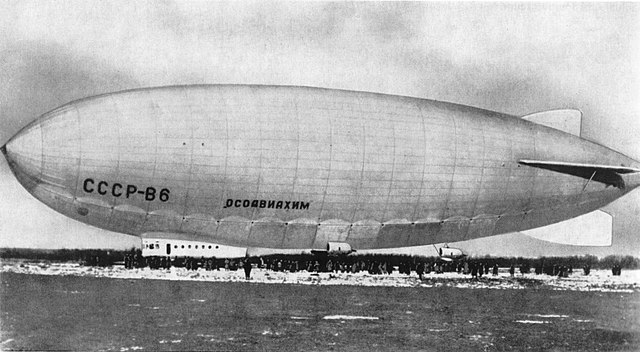
\includegraphics[width=\linewidth]{./chapter/aircraft/foto_of_airship.jpg}}
    }
	\caption{Airship.}
	\labfig{fig:airship_question_answers_aircraft_en}
\end{marginfigure}

Airship. 

Question from page~\pageref{question:aircraft_question_4}.

%%%%%%%%%%%%%%%%%%%%%%%%%%%%answer_5%%%%%%%%%%%%%%%%%%%%%%

\begin{exercise}%
\label{answer:aircraft_question_airship_2_en}
Which aircraft is shown in Fig. \ref{fig:airship_question_answers_aircraft_en}?

\end{exercise}

The aircraft shown in Fig. \ref{fig:airship_question_aircraft_en} is an airship. 
The answer to the question can also be obtained by running the following SPARQL-request (listing \ref{lst:aircraft_airship_photo_lst_en})

\begin{lstlisting}[ language=SPARQL, breaklines=true, 
                    caption={Airship images\\\hspace{\textwidth}
                        SPARQL query: \href{https://w.wiki/rg4}{w.wiki/rg4}
                        },
                    label=lst:aircraft_airship_photo_lst_en,
                    texcl 
                    ]
#defaultView:ImageGrid
SELECT ?airship ?airshipLabel ?image
WHERE
{
    ?airship wdt:P31 wd:Q133585. # instance of airship
  	?airship wdt:P18 ?image # image airship
    SERVICE wikibase:label { bd:serviceParam wikibase:language "en" }
}
\end{lstlisting}

Question from page~\pageref{question:aircraft_question_5}.

%%%%%%%%%%%%%%%%%%end_answers_aircraft%%%%%%%%%%%%%%%%%%%%%%%%%%%%%%


\section{From towns to cities with millions of inhabitants}
\labsec{answer-towns}

\begin{exercise}%
    \label{answer:cities_geographic_objects}
Which of the following cities were named after toponyms?
\begin{itemize}
\item \href{https://w.wiki/pzi}{Tolyatti}
\item \href{https://w.wiki/pzj}{Tula}
\item \href{https://w.wiki/pzk}{Chernyakhovsk}
\item \href{https://w.wiki/pzm}{Kurilsk}
\item \href{https://w.wiki/pzn}{Vologda}
\item \href{https://w.wiki/pzo}{Obninsk}
\end{itemize}
\end{exercise}

Tula, Kurilsk and Vologda were named after the following toponyms: Tulitsa river, \href{https://w.wiki/qqJ}{Kuril Islands}, \href{https://w.wiki/qqK}{Vologda river}. The answer to the question can also be obtained by running the following SPARQL query (Listing \ref{lst:cities_geographic_objects}). The \href{https://www.wikidata.org/wiki/Property:P138}{named after (P138)} property value shows which Wikidata object the city was named after.
    
\index{SPARQL!FILTER!Cities named after toponyms}
\begin{lstlisting}[ language=SPARQL, 
                    caption={Cities named after toponyms.\\\hspace{\textwidth}
                        SPARQL query: \href{https://w.wiki/otn}{w.wiki/otn}
                        },
                    label=lst:cities_geographic_objects,
                    texcl 
                    ]
SELECT ?city ?cityLabel ?namedAfterLabel ?whatIsItLabel WHERE {
	?city wdt:P31/wdt:P279* wd:Q7930989. # "city/town" subclasses
	?city wdt:P138 ?namedAfter. # with property "named after"
	?namedAfter wdt:P31 ?whatIsIt. # which is instance of
	FILTER(?city = wd:Q1341 || ?city = wd:Q2770 || ?city = wd:Q5655 
		|| ?city = wd:Q156046 || ?city = wd:Q1957 || ?city = wd:Q175651)
	SERVICE wikibase:label {bd:serviceParam wikibase:language "en"}
}
\end{lstlisting}%

See question on page~\pageref{question:cities_geographic_objects}.

\marginnote[-2.0cm]{
Let's explain the second line of the script in the Listing \ref{lst:cities_geographic_objects}, that is, the construction wdt:P31/wdt:P279*, followed by a Wikidata object that combines \wdqName{city}{515} and \wdqName{town}{3957}, and is called \mbox{\wdqName{city/town}{7930989}}. If it doesn't matter what certain type of city the Wikidata object belongs to, you can use a construction with subclasses, specifying the only class relative to which the search will be performed. This construction is discussed in more detail in the section  ``Wikidata completeness and disadvantages'', in the text before Listing \ref{lst:example_subclasses_city} on page \pageref{lst:example_subclasses_city}.
}

\begin{exercise}%
    \label{answer:cities_over_400_age}
Which of the following cities were founded more than 400 years ago: \href{https://w.wiki/pzt}{Moscow}, \href{https://w.wiki/pzu}{Sarov}, \href{https://w.wiki/pzx}{Kazan}, \href{https://w.wiki/pzy}{Astrakhan}, \href{https://w.wiki/pzz}{Samara}, \href{https://w.wiki/pz$}{Voronezh}?
\end{exercise}

Kazan (1005 year), Moscow (1147), Astrakhan (1558), Voronezh (1586) and Samara (1586) were founded more than 400 years ago. Sarov, which had been founded in 1691, turned out to be the youngest city. The answer to the question can also be obtained by running the following SPARQL query (Listing \ref{lst:cities_over_400_age}). The \href{https://www.wikidata.org/wiki/Property:P571}{inception (P571)} property value contains the date the city was founded.

\index{SPARQL!FILTER!Cities founded more than 400 years ago}
\index{SPARQL!YEAR!Cities founded more than 400 years ago}
\begin{lstlisting}[ language=SPARQL, 
                    caption={Cities founded more than 400 years ago.\\\hspace{\textwidth}
                        SPARQL query: \href{https://w.wiki/t5v}{w.wiki/t5v}
                        },
                    label=lst:cities_over_400_age,
                    texcl 
                    ]
SELECT ?city ?cityLabel (YEAR(?inceptionDate) AS ?year) WHERE {
	?city wdt:P31/wdt:P279* wd:Q7930989. # "city/town" subclasses
	?city wdt:P17 wd:Q159. # belonging to Russia
	?city wdt:P571 ?inceptionDate. # with property "inception"  
	FILTER (YEAR(?inceptionDate) < 1620). # 2020 - 400 years
	FILTER(?city = wd:Q649 || ?city = wd:Q193522 || ?city = wd:Q900
		|| ?city = wd:Q3927 || ?city = wd:Q894 || ?city = wd:Q3426)
	SERVICE wikibase:label {bd:serviceParam wikibase:language "en"}
}
GROUP BY ?city ?cityLabel ?inceptionDate
ORDER BY ASC(?year)
\end{lstlisting}%

\marginnote[-3.5cm]{
Which lines in the Listing \ref{lst:cities_over_400_age} should be commented out for:
\begin{itemize}
	\item[a)] getting a list of Russian cities which were founded more than 400 years ago?
	\item[b)] getting a list of world cities which were founded at the same years?
\end{itemize}
}

\marginnote{
Can the ?year variable be negative in the Listing \ref{lst:cities_over_400_age}? Why?
}

The Wikidata object \wdqName{Moscow}{649} has ``unknown value'' of \href{https://www.wikidata.org/wiki/Property:P571}{inception} property with the \href{https://www.wikidata.org/wiki/Property:P1326}{latest date} qualifier = April 4, 1147. Probably for this reason, in the Listing \ref{lst:cities_over_400_age} the ?year variable takes an empty value for Moscow, and Moscow is mistakenly not included in the list of correct answers. Thus, to extract the year 1147, it is necessary to modify the existing script, which we will leave to the reader.

\marginnote[-1.0cm]{
About types of data and sets of properties related to date and time, see \href{https://w.wiki/NdT}{Help:Dates}.
}

See question on page~\pageref{question:cities_over_400_age}.

\begin{exercise}%
    \label{answer:cities_flags}
Which city does the flag in \reffig{fig:flag_question_city} belong to?
\end{exercise}

The flag in \reffig{fig:flag_question_city} belongs to \href{https://w.wiki/qqN}{Karabulak}. The answer to the question can also be obtained by running the following SPARQL query (Listing \ref{lst:cities_flags}). The \href{https://www.wikidata.org/wiki/Property:P41}{flag image (P41)} property value contains the image of the city flag.

\index{SPARQL!FILTER!Cities flags}
\begin{lstlisting}[ language=SPARQL, 
                    caption={Cities flags.\\\hspace{\textwidth}
                        SPARQL query: \href{https://w.wiki/t5s}{w.wiki/t5s}
                        },
                    label=lst:cities_flags,
                    texcl 
                    ]
#defaultView:ImageGrid
SELECT ?city ?cityLabel ?flag ?countryLabel WHERE {
	?city wdt:P31/wdt:P279* wd:Q7930989. # "city/town" subclasses
	?city wdt:P17 wd:Q159. # belonging to Russia
	?city wdt:P41 ?flag. # with filled property "flag"
	SERVICE wikibase:label {bd:serviceParam wikibase:language "en"}
}
\end{lstlisting}%

See question on page~\pageref{question:cities_flags}.

\section{Analysis of aspects of modern countries}
\labsec{answer-languages}
\begin{exercise}
\label{answer:population_density}
Identify the countries of Asia by flags and list them in ascending order of population density (fig. ~\ref{fig:flag_kor}, ~\ref{fig:flag_mongolia}, ~\ref{fig:flag_singapore}, ~\ref{fig:flag_israel}).
\end{exercise}

\begin{enumerate}
\item Mongolia (\num{1.96} people km\begin{math}^2\end{math}), (fig. ~\ref{fig:flag_mongolia});
\item Israel (\num{437.79} people km\begin{math}^2\end{math}), (fig. ~\ref{fig:flag_israel});
\item Korea (\num{513.14} people km\begin{math}^2\end{math}), (fig. ~\ref{fig:flag_kor});
\item Singapore (\num{8189.30} people km\begin{math}^2\end{math}), (fig. ~\ref{fig:flag_singapore}).
\end{enumerate}

The answer to the question can also be obtained by running the following SPARQL query (Listing \ref{lst:population_density}).

\begin{lstlisting}[ language=SPARQL, 
caption={\href{https://w.wiki/vLJ}{
		Population density in Asia}\protect\footnotemark},
label=lst:population_density
]
# Population density in Asian countries
SELECT ?country ?countryLabel ?flag ?area ?population 
(?population / ?area as ?populationDensity)
{
	?country p:P31 [ps:P31 wd:Q6256].# this is a country
	?country wdt:P30 wd:Q48 .   # on the Asian continent 
	?country wdt:P41 ?flag .    # has flag
	?country wdt:P2046 ?area .  # has area
	?country wdt:P1082 ?population. # has population  
	SERVICE wikibase:label {bd:serviceParam wikibase:language "en"}
}
ORDER BY DESC(?populationDensity)
\end{lstlisting}

See question on page~\pageref{question:population_density}.
%%%%%%%%%%%%%%%%%%%%%%%%%%%%%%%%%%%%%%%%%%%%
\begin{exercise}
\label{answer:old_countries}

Find the states that have existed the longest.

\end{exercise}

The result of the script (Listing \ref{lst:old_countries}) will be a list of empires and small countries that have disappeared from the face of the earth. Two and a half thousand years and more, only seven states existed: \href{https://w.wiki/vAT}{Ugarit} (4810 years), \href{https://w.wiki/vAU}{Tamla} (3740 years), \href{https://w.wiki/vAX}{Ancient Egypt} (3544 years), \href{https://w.wiki/vAY}{Maya} (3521), \href{ https://w.wiki/vAZ}{Idalion} (2550), \href{https://w.wiki/vAb}{Meroite Kingdom} (2529) and the city-state \href{https://w.wiki/vAf}{Dilmun} (2500 years old).

\begin{lstlisting}[ language=SPARQL, 
caption={\href{https://w.wiki/tYc}{List of historical countries sorted by inception date}\protect\footnotemark},
label=lst:old_countries
]
# List of historical countries sorted by inception date
SELECT ?country ?countryLabel 
(MIN(?start) AS ?min_year)
(MAX(?end)   AS ?max_year) 
(?max_year - ?min_year as ?age)
WHERE
{
	?country p:P31 [ps:P31 wd:Q3024240]. # instance of a historical country
	
	FILTER EXISTS {?country wdt:P571 []}.# skip countries without inception date
	FILTER EXISTS {?country wdt:P576 []}.# skip countries without dissolution date
	
	OPTIONAL {?country p:P571 [ps:P571 ?inception].}# any inception date
	OPTIONAL {?country p:P576 [ps:P576 ?dissolution].}# any dissolution date
	
	BIND(YEAR(?inception) AS ?start)
	BIND(YEAR(?dissolution) AS ?end)  
	SERVICE wikibase:label { bd:serviceParam wikibase:language "ru,[AUTO_LANGUAGE],en" }
}
GROUP BY ?country ?countryLabel ?min_year ?max_year ?age
ORDER BY DESC(?age)
\end{lstlisting}

See question on page~\pageref{question:old_countries}.
%%%%%%%%%%%%%%%%%%%%%%%%%%%%%%%%%%%%%%%%%%%%
\begin{exercise}
\label{answer:official_languages}
Which of these languages are official in \href{https://en.wikipedia.org/wiki/Russia}{Russia}?
\begin{itemize}
\item \href{https://en.wikipedia.org/wiki/Abaza_language}{Abaza};
\item \href{https://en.wikipedia.org/wiki/Moksha_language}{Moksha};
\item \href{https://en.wikipedia.org/wiki/Erzya_language}{Erzya};
\item \href{https://en.wikipedia.org/wiki/Belarusian_language}{Belarusian}.
\end{itemize}
\end{exercise}

The official languages of Russia are the Abaza, Moksha and Erzyan languages. The answer to the question can also be obtained by running the following SPARQL query (Listing \ref{lst:official_languages}).

\begin{lstlisting}[ language=SPARQL, 
caption={\href{https://w.wiki/vLK}{Official languages in Russia}\protect\footnotemark},
label=lst:official_languages
]
# Official languages in Russia
SELECT ?lanquage ?lanquageLabel
WHERE
{ # Russia has the official language
	wd:Q159 p:P37 [ps:P37 ?lanquage].
	SERVICE wikibase:label {bd:serviceParam wikibase:language "en"}
} ORDER BY ?lanquageLabel
\end{lstlisting}

See question on page~\pageref{question:official_language}.
%%%%%%%%%%%%%%%%%%%%%%%%%%%%%%%%%%%%%%%%%%%%
\begin{exercise}
\label{answer:administrative_territorial}

Latvia has 119, Thailand has 77, Denmark has 5, and Russia has 81. What are we talking about?
\begin{itemize}
\item Is a number of cities with a population of over one million?
\item Is a number of higher education institutions?
\item Is a number of administrative units?
\item Is a number of official languages?
\end{itemize}

\end{exercise}

We are talking about the number of administrative-territorial units in each country. The answer to the question can also be obtained by running the following SPARQL query (Listing \ref{lst:administrative_territorial}).

\begin{lstlisting}[ language=SPARQL, 
caption={\href{https://w.wiki/vL6}{Countries sorted by number of administrative territories country}\protect\footnotemark},
label=lst:administrative_territorial
]
# Countries sorted by number of administrative territories
SELECT ?country ?countryLabel  (count(*) as ?count)
WHERE
{
	?country p:P31 [ps:P31 wd:Q6256].# is a country
	?country wdt:P150 []. # has some administrative territory
	SERVICE wikibase:label { bd:serviceParam wikibase:language "en" }
}
GROUP BY ?country ?countryLabel
ORDER BY DESC(?count)
\end{lstlisting}

See question on page~\pageref{question:administrative_territorial}.

%%%%%%%%%%%%%%%%%%operating systems%%%%%%%%%%%%%%%%%%%%%%

\section{Programming languages for operating systems}
\labsec{answer-operating-systems}

% question 1
\begin{exercise}%
	\label{answer:os_base}
	Choose operating system 
	\href{https://w.wiki/n8U}{Debian},
	\href{https://w.wiki/n8V}{Android},
	\href{https://w.wiki/n8W}{Ubuntu} or
	\href{https://w.wiki/n8X}{Linux kernel}
	which has the most count of based on it other operating systems.	
\end{exercise}

\href{https://w.wiki/n8W}{Ubuntu}  has the largest number of operating systems developed, namely 11. The answer to this question can also be obtained by running the following SPARQL query (listing \ref{lst:os_base}).

\begin{lstlisting}[ language=SPARQL, breaklines=true, 
	caption={List of bases of operating systems\\\hspace{\textwidth}
		SPARQL query: \href{https://w.wiki/uLR}{https://w.wiki/uLR}
	},
	label=lst:os_base,
	texcl 
	]
SELECT ?baseLabel (COUNT(*) AS ?count)
WHERE
{
	?os wdt:P31 wd:Q9135. # is instance of operating system
	?os wdt:P144 ?base.   # is based on ?base
SERVICE wikibase:label { bd:serviceParam wikibase:language "en"}
}
GROUP BY ?baseLabel
ORDER BY DESC(?count) ASC(?baseLabel)
\end{lstlisting}

Question from page~\pageref{lst:base_of_operating_systems}.

% question 2
\begin{exercise}
	\label{answer:what_system_created}
	Which of operating systems
	\href{https://w.wiki/n8P}{Newton OS},
	\href{https://w.wiki/n8Q}{Ubuntu Touch} or
	\href{https://w.wiki/n8R}{JavaOS} is developed by
	\href{https://w.wiki/n8S}{Apple}?	
\end{exercise}
\href{https://w.wiki/n8S}{Apple}  developed  \href{https://w.wiki/n8P}{Newton OS}. You can also get the answer to the question by running the following SPARQL query (Listing \ref{lst:os_creators}).

\begin{lstlisting}[ language=SPARQL, breaklines=true, 
	caption={Ooperating systems developers\\\hspace{\textwidth}
		SPARQL query: \href{https://w.wiki/vMK}{https://w.wiki/vMK}
	},
	label=lst:os_creators,
	texcl 
	]
SELECT ?os ?osLabel ?developer ?developerLabel 
WHERE {
	?os wdt:P31 wd:Q9135. # instance of operating system
	OPTIONAL { ?os wdt:P178 ?developer. }
SERVICE wikibase:label { bd:serviceParam wikibase:language "en"}
}
\end{lstlisting}

Question from page~\pageref{lst:inception_time_of_operating_systems}.

% exercise 1
\begin{exercise}
	\label{answer:os_and_developers}
	Create list operating systems with information about their developers.
\end{exercise}
The list of operating system developers can be obtained by executing the following SPARQL query \ref{lst:os_creators_2}.

\begin{lstlisting}[ language=SPARQL, breaklines=true, 
	caption={Operating systems developers\\\hspace{\textwidth}
		SPARQL query: \href{https://w.wiki/vMT}{https://w.wiki/vMT}
	},
	label=lst:os_creators_2,
	texcl 
	]
SELECT ?os ?osLabel ?developer ?developerLabel
WHERE {
	?os wdt:P31 wd:Q9135. # os is instance of operating system
	?os wdt:P178 ?developer. # os developed by developer
SERVICE wikibase:label { bd:serviceParam wikibase:language "en"}
}
\end{lstlisting}

Question from page~\pageref{tasks:operating_system_tasks}.

% exercise 2
\begin{exercise}
	\label{answer:os_and_logos}
	Find list operating systems with their logos
\end{exercise}
The list of operating system logos can be obtained by executing the following SPARQL query \ref{lst:os_and_logos}.

\begin{lstlisting}[ language=SPARQL, breaklines=true, 
	caption={Logos of operating systems\\\hspace{\textwidth}
		SPARQL query: \href{https://w.wiki/vMW}{https://w.wiki/vMW}
	},
	label=lst:os_and_logos,
	texcl 
	]
SELECT ?os ?osLabel ?image 
WHERE {
	?os wdt:P31 wd:Q9135.
	?os wdt:P18 ?image.
SERVICE wikibase:label { bd:serviceParam wikibase:language "en"}
}
\end{lstlisting}

Question from page~\pageref{tasks:operating_system_tasks}.

% exercise 3
\begin{exercise}
	\label{answer:os_country}
	Find countries of origin of operating systems
\end{exercise}
The list of countries of origin of operating systems can be obtained by executing the following SPARQL query \ref{lst:os_development_country}.

\begin{lstlisting}[ language=SPARQL, breaklines=true, 
	caption={Countries where developed operating systems\\\hspace{\textwidth}
		SPARQL query: \href{https://w.wiki/vMa}{https://w.wiki/vMa}
	},
	label=lst:os_development_country,
	texcl 
	]
SELECT ?os ?osLabel ?country ?countryLabel
WHERE {
	?os wdt:P31 wd:Q9135.
	?os wdt:P495 ?country.
SERVICE wikibase:label { bd:serviceParam wikibase:language "en"}
}
\end{lstlisting}

Question from page~\pageref{tasks:operating_system_tasks}.

% exercise 4
\begin{exercise}
	\label{answer:os_and_bases}
	Create a script that creates a tree diagram. Top-level lines should contain operating systems. When ``deploying'', we should see a list of operating systems that were based on the system from the top-level line.
\end{exercise}
To get a tree of operating systems at the top level, and operating systems based on them, at the bottom, you can run the following SPARQL query \ref{lst:os_and_bases}.

\begin{lstlisting}[ language=SPARQL, breaklines=true, 
	caption={Operating systems tree and their basics\\\hspace{\textwidth}
		SPARQL query: \href{https://w.wiki/vMb}{https://w.wiki/vMb}
	},
	label=lst:os_and_bases,
	texcl 
	]
#defaultView:Tree
SELECT ?base ?baseLabel ?baseImage ?baseLogoImage
?os ?osLabel ?osImage ?osLogoImage
WHERE
{
	?os wdt:P31 wd:Q9135. 
	?os wdt:P144 ?base.
	OPTIONAL { ?base wdt:P18 ?baseImage. }
	OPTIONAL { ?base wdt:P154 ?baseLogoImage. }
	OPTIONAL { ?os wdt:P18 ?osImage. }
	OPTIONAL { ?os wdt:P154 ?osLogoImage. }
SERVICE wikibase:label { bd:serviceParam wikibase:language "en"}
}
\end{lstlisting}

Question from page~\pageref{tasks:operating_system_tasks}.

%%%%%%%%%%%%%%%%%%end operating systems%%%%%%%%%%%%%%%%%%%%%%%%%%%%%%

\section{Programming languages and its creators}
\labsec{answer-languages}
\begin{exercise}
    \label{answer:prog_lang_1}
Correlate a programming language and its developer.
	\begin{tabular}{ll}
		Developer & Language\\
		\hline
		J. Ichbiah & \href{https://www.wikidata.org/wiki/Q154755}{Ada}\\
		C. Moore & \href{https://www.wikidata.org/wiki/Q275472}{Forth}\\
		J. Armstrong & \href{https://www.wikidata.org/wiki/Q334879}{Erlang}\\
	\end{tabular}
\end{exercise}
    The Ada programming language was developed by Jean Ichbiah, Forth was developed by Charles H. Moore, and the creator of Erlang is believed to be Joe Armstrong. The answer to the question can also be obtained by running the following SPARQL query (listing \ref{lst:prog_lang_answer_1}). 
	\begin{lstlisting}[language=SPARQL, caption={{Programming languages developers}\protect\footnotemark}, label=lst:prog_lang_answer_1]
		SELECT ?item_label ?developer_label
		WHERE
		{
		 ?item wdt:P31 wd:Q9143
		 ; rdfs:label ?item_label. 
		 ?item wdt:P178 ?developer.
		 ?developer rdfs:label ?developer_label.
		 
		 FILTER (LANG(?item_label) = "en"). 
		 FILTER (LANG(?developer_label) = "en"). 
		}
		ORDER BY DESC (?item_label)
	\end{lstlisting}
SPARQL query: \href{https://w.wiki/kfZ}{https://w.wiki/kfZ}

Question from page~\pageref{question:prog_lang_1}.


\begin{exercise}
    \label{answer:prog_lang_2}
Which image is the programming language logo \href{https://www.wikidata.org/wiki/Q513238}{LOLCODE}:
    \begin{tabular}{c c c c}

\includegraphics[width=2cm]{./chapter/programming_language/task_2_logo_1.PNG} & 
\includegraphics[width=2cm]{./chapter/programming_language/task_2_logo_2.PNG} & 
\includegraphics[width=2cm]{./chapter/programming_language/task_2_logo_3.PNG} & 
\includegraphics[width=2cm]{./chapter/programming_language/task_2_logo_4.PNG}
	\end{tabular}
\end{exercise}
    The third picture is the logo of the LOLCODE programming language. The answer to the question can also be obtained by running the following SPARQL query (listing \ref{lst:prog_lang_answer_1}). 
	\begin{lstlisting}[language=SPARQL, caption={{Programmers languages logos}\protect\footnotemark}, label=lst:prog_lang_answer_1]
		#defaultView:ImageGrid
		SELECT ?item_label ?image
		WHERE
		{
		 ?item wdt:P31 wd:Q9143 # instances of programming language
		 ; rdfs:label ?item_label. 
		 ?item wdt:P154 ?image. # image
		 	
		 	FILTER (lang(?item_label) = "en")
}
	\end{lstlisting}
SPARQL query: \href{https://w.wiki/kfd}{https://w.wiki/kfd}

Question from page~\pageref{question:prog_lang_2}.


\begin{exercise}
    \label{answer:prog_lang_3}
Fill the gaps.

\href{https://www.wikidata.org/wiki/Q83303}{Fortran} ranks first in terms of the number of its dialects. Their number reaches about \underline{\hspace{1cm}}. In second place is \href{https://www.wikidata.org/wiki/Q132874}{Lisp}, it has \underline{\hspace{1cm}} dialects. The third place is shared by\href{https://www.wikidata.org/wiki/Q597330}{Standard ML} and \href{https://www.wikidata.org/wiki/Q633894}{Object Pascal} with \underline{\hspace{1cm}} dialects.
\end{exercise}
 It is believed that Fortran has 8 to 12 dialects, Lisp has 6 dialects, and Standard ML and Object Pascal have 3 dialects.
    
Question from page~\pageref{question:prog_lang_3}.



%%%%%%%%%%%%%%%%%%%  Ship chapter  %%%%%%%%%%%%%%%%%%

\begin{exercise}
	\label{answer:ship_1}
	The figure shows the most famous \href{https://en.wikipedia.org/wiki/Destroyer}{destroyer} \href{https://en.wikipedia.org/wiki/Gnevny-class_destroyer}{project 7}, awarded the title of "Guards", name it.
	  {
		\setlength{\fboxsep}{0pt}%
		\setlength{\fboxrule}{1pt}%
		\fcolorbox{gray}{gray}{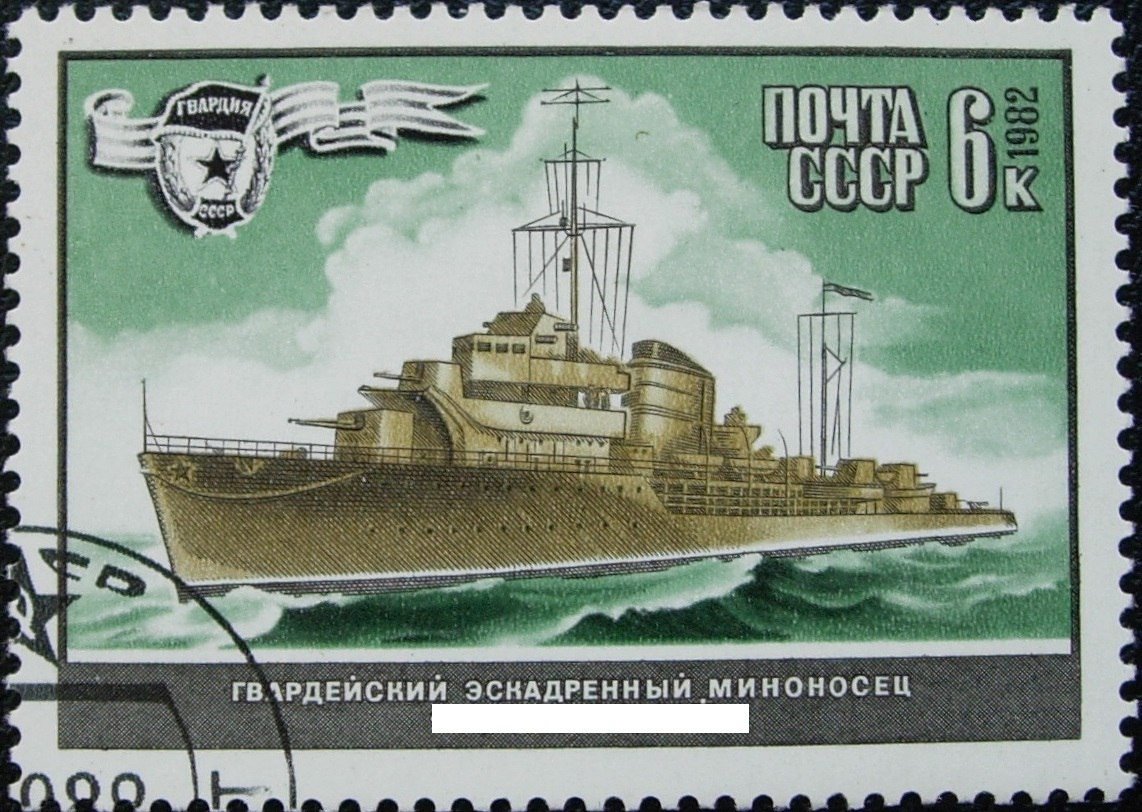
\includegraphics{chapter/ship/Secret_Grem_ship.jpg}}
	  }
\end{exercise}
Answer: \href{https://en.wikipedia.org/wiki/Soviet_destroyer_Gremyashchy_(1937)}{Soviet destroyer Gremyashchy (1937)}.



\begin{exercise}
	\label{answer:ship_2}
	Based on the graph of the dependence of ships and military operations (Fig. \ref{fig:ships_by_country_and_conflict}), which country has the most values of wars associated with ships?
	\begin{itemize}
		\item \href{https://www.wikidata.org/wiki/Q15180}{Soviet Union}
		\item \href{https://www.wikidata.org/wiki/Q159}{Russia}
		\item \href{https://www.wikidata.org/wiki/Q34266}{Russian Empire}
	\end{itemize}
\end{exercise}
Answer: Russia.


\begin{exercise}
	\label{answer:ship_3}
	Based on the graph of the dependence of ships and military operations (Fig. \ref{fig:ships_by_country_and_conflict}), which war accounts for most of the values of ships?
	\begin{itemize}
	  \item \href{https://www.wikidata.org/wiki/Q159950}{Russo-Japanese War}
	  \item \href{https://www.wikidata.org/wiki/Q362}{World War II}
	  \item \href{https://www.wikidata.org/wiki/Q254106}{Crimean War}
	\end{itemize}
\end{exercise}
Answer: World War II.



\begin{exercise}
	\label{answer:ship_ex_1}
	Find the "Guinness ship" (to choose from: the largest, the longest, the most capacious).
\end{exercise}

Possible solution: \href{https://en.wikipedia.org/wiki/Seawise_Giant}{Seawise Giant}

Other possible solutions from Wikidata. The data may differ beacouse of imcopmlintess of wikidata objects' properties, see the listings \ref{lst:long_ship} and \ref{lst:wide_ship}.
\begin{lstlisting}[ language=SPARQL, caption={{\href{https://w.wiki/ugH}{The longest wikidata ship. SPARQL-querry: \href{https://w.wiki/ugH}{https://w.wiki/ugH}. Ship in result: \href{https://www.wikidata.org/wiki/Q48817670}{NMS Mircea}, January 2021, length \num{36} m.}}\protect\footnotemark}, label=lst:long_ship, ]
SELECT ?ship ?shipLabel ?length
WHERE
{
	?ship wdt:P31 wd:Q11446;        # instance of ship
		  wdt:P2043 ?length.
	  
	SERVICE wikibase:label { bd:serviceParam wikibase:language "en"}
}
ORDER BY DESC(?length) LIMIT 1
\end{lstlisting}

\begin{lstlisting}[ language=SPARQL, caption={{\href{https://w.wiki/ugG}{The widest wikidata ship. SPARQL-querry: \href{https://w.wiki/ugG}{https://w.wiki/ugG}. Ship in result: \href{https://www.wikidata.org/wiki/Q1156392}{Project Habakkuk}, January 2021, width \num{180} m.}}\protect\footnotemark}, label=lst:wide_ship, ]
SELECT ?ship ?shipLabel ?beam
WHERE
{
	?ship wdt:P31 wd:Q11446;        # instance of ship
		  wdt:P2261 ?beam.
	  
	SERVICE wikibase:label { bd:serviceParam wikibase:language "en"}
}
ORDER BY DESC(?beam) LIMIT 1
\end{lstlisting}


\begin{exercise}
	\label{answer:ship_ex_2}
	Output pictures of those ships, about which the film were shot. If there are no such, then those ships, about which the books were written.\\

\end{exercise}
Possible answer:\\
{
	\setlength{\fboxsep}{0pt}%
	\setlength{\fboxrule}{1pt}%
	\fcolorbox{gray}{gray}{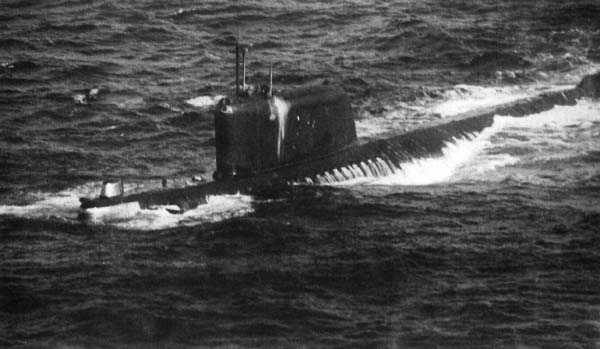
\includegraphics{chapter/ship/K-19.jpg}}
}

Submarine \href{https://en.wikipedia.org/wiki/Soviet_submarine_K-19}{K-19} was filmed in \href{https://en.wikipedia.org/wiki/K-19:_The_Widowmaker}{K-19: The Widowmaker}.  Source: \href{https://commons.wikimedia.org/wiki/File:K-19.jpg}{https://commons.wikimedia.org/wiki/File:K-19.jpg}, Norman Polamar Cold War Submarines.



\begin{exercise}
	\label{answer:ship_ex_3}
	Find \href{https://en.wikipedia.org/wiki/List_of_museum_ships}{the museum ship}.
\end{exercise}

Solution is in listing \ref{lst:museum_ship}.

\begin{lstlisting}[ language=SPARQL, caption={{\href{https://w.wiki/ugG}{Museum ships in wikidata}. SPARQL-querry: \href{https://w.wiki/uhG}{https://w.wiki/uhG.}}\protect\footnotemark}, label=lst:museum_ship, ]
SELECT ?ship ?shipLabel
WHERE
{
	?ship wdt:P31 wd:Q575727
			   
	SERVICE wikibase:label { bd:serviceParam wikibase:language "en"}
}
\end{lstlisting}
		
